%Here you can see how to include an image in your document.
%
%\begin{sidewaysfigure}
%\centering
%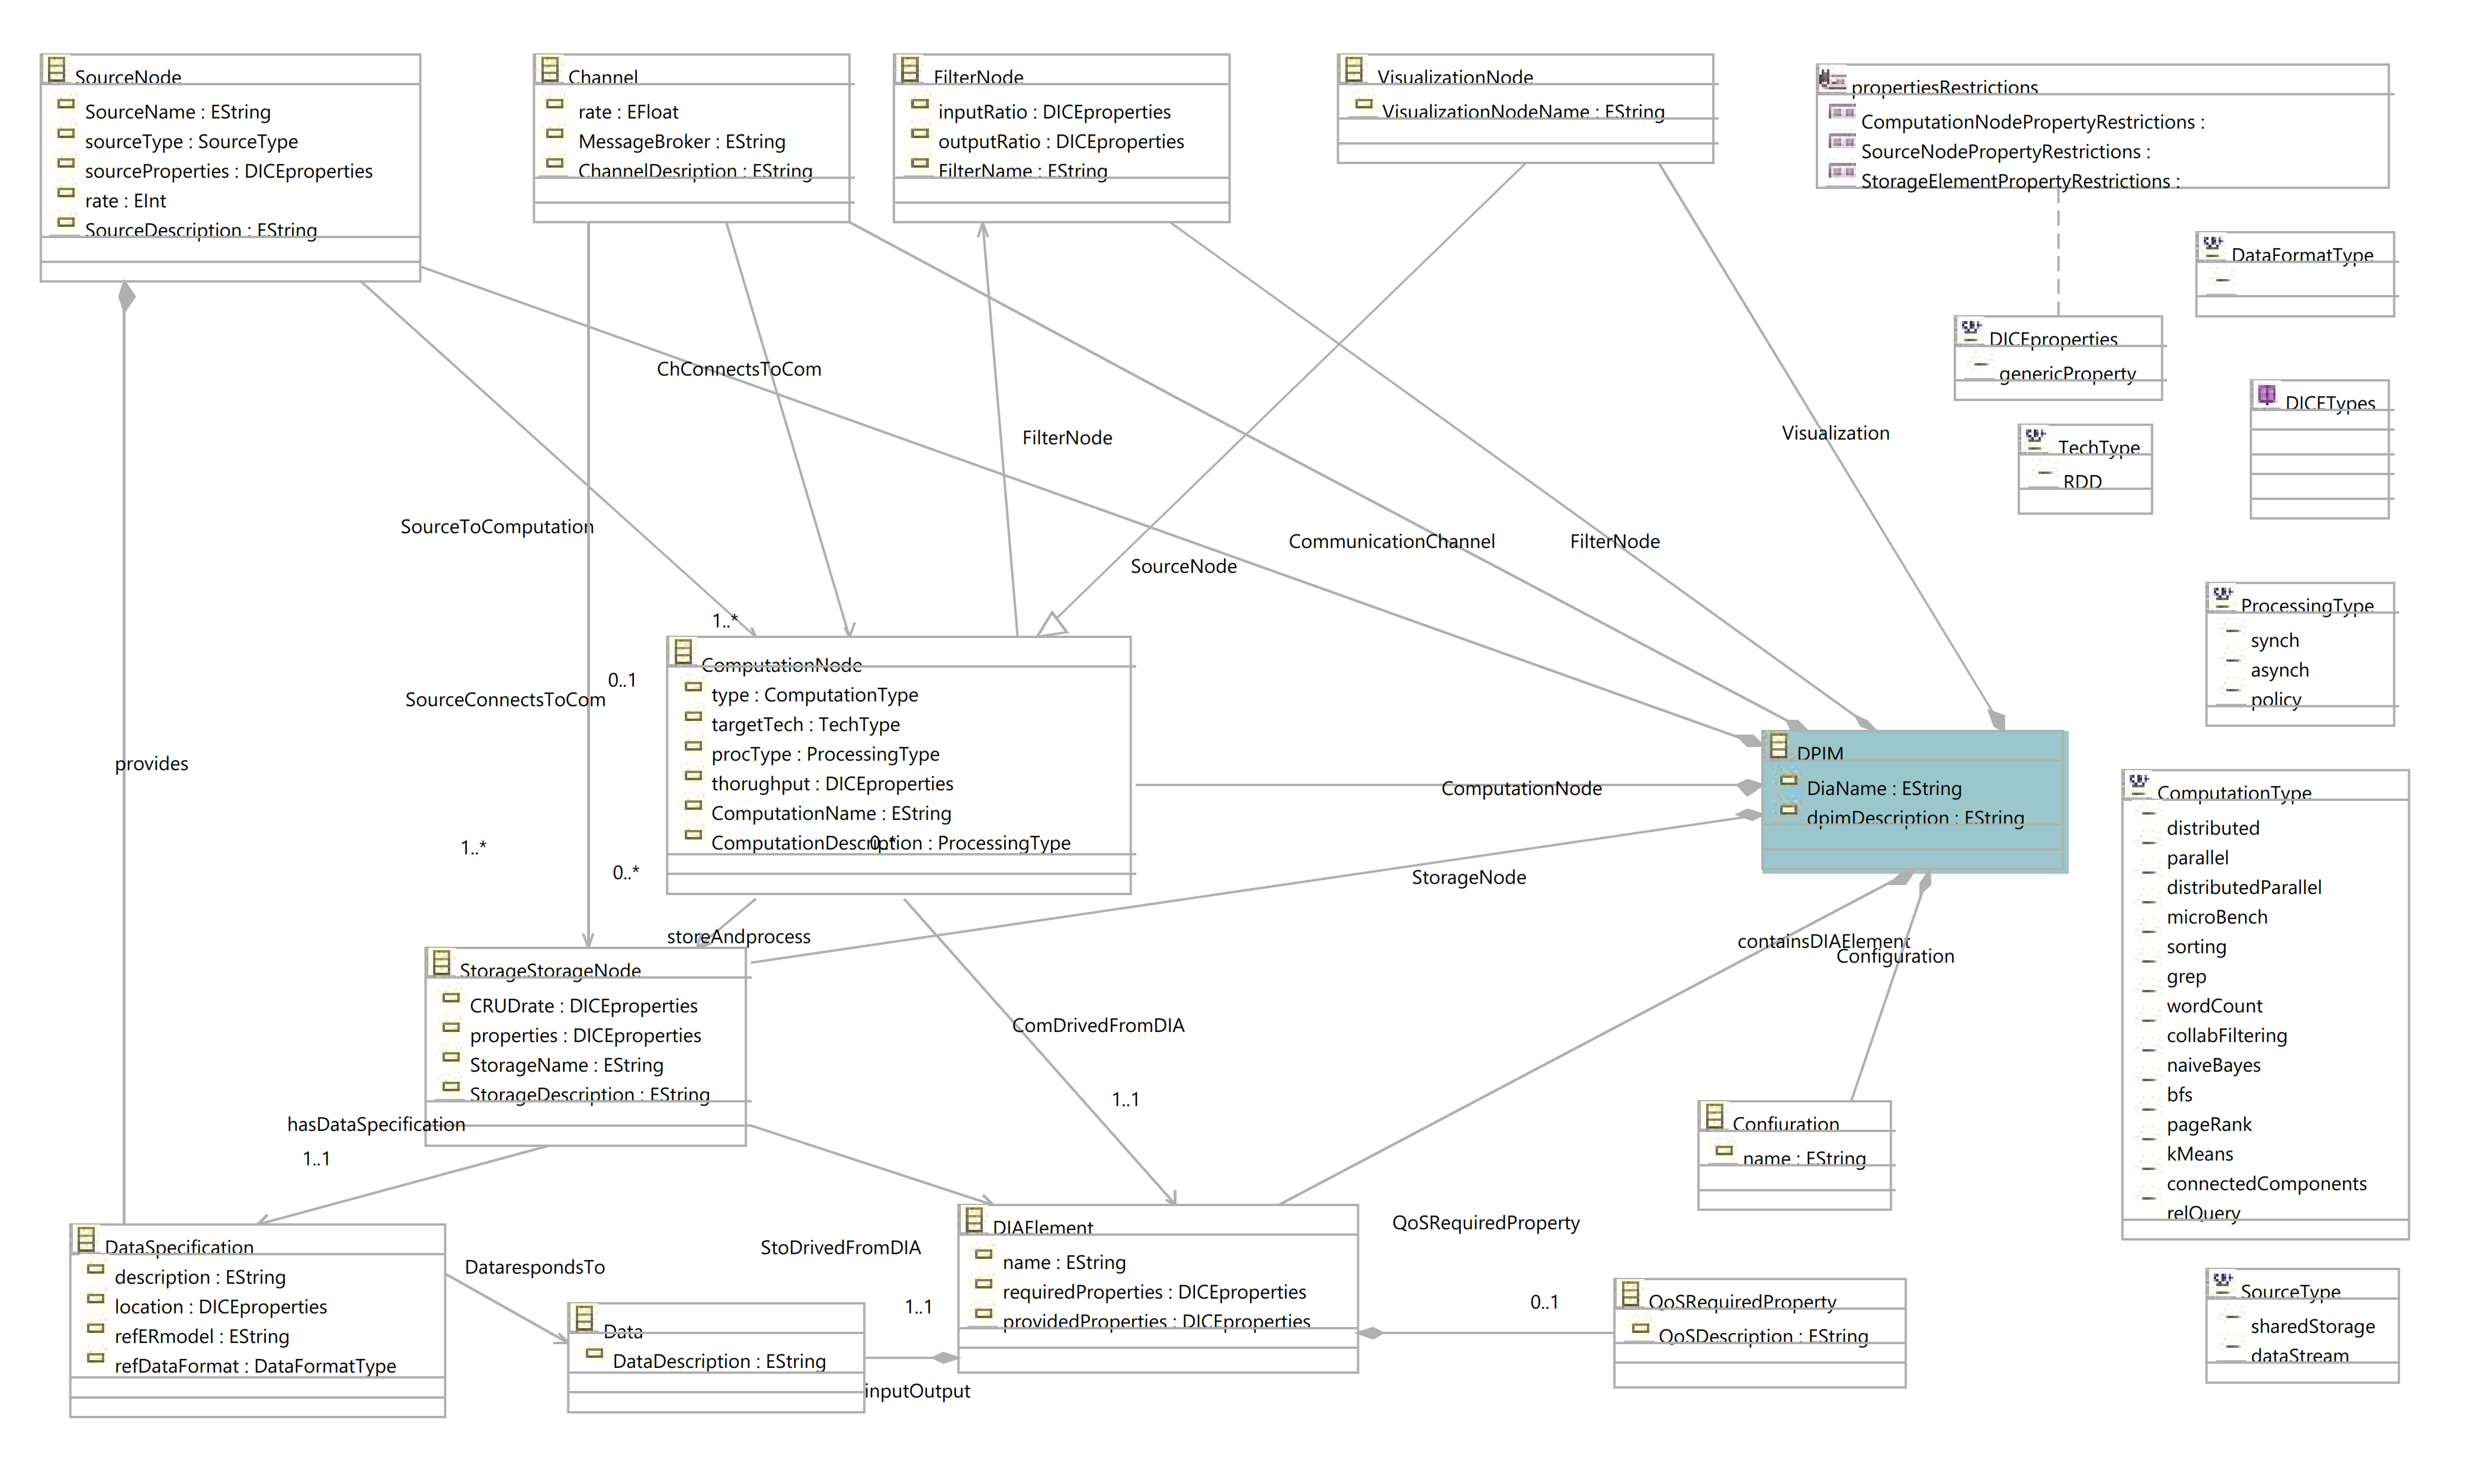
\includegraphics[width=\textwidth]{Images/11.png}
%\caption{\label{fig:metamodel}DICE DPIM metamodel.}
%\end{sidewaysfigure}

%\begin{figure}
%\centering
%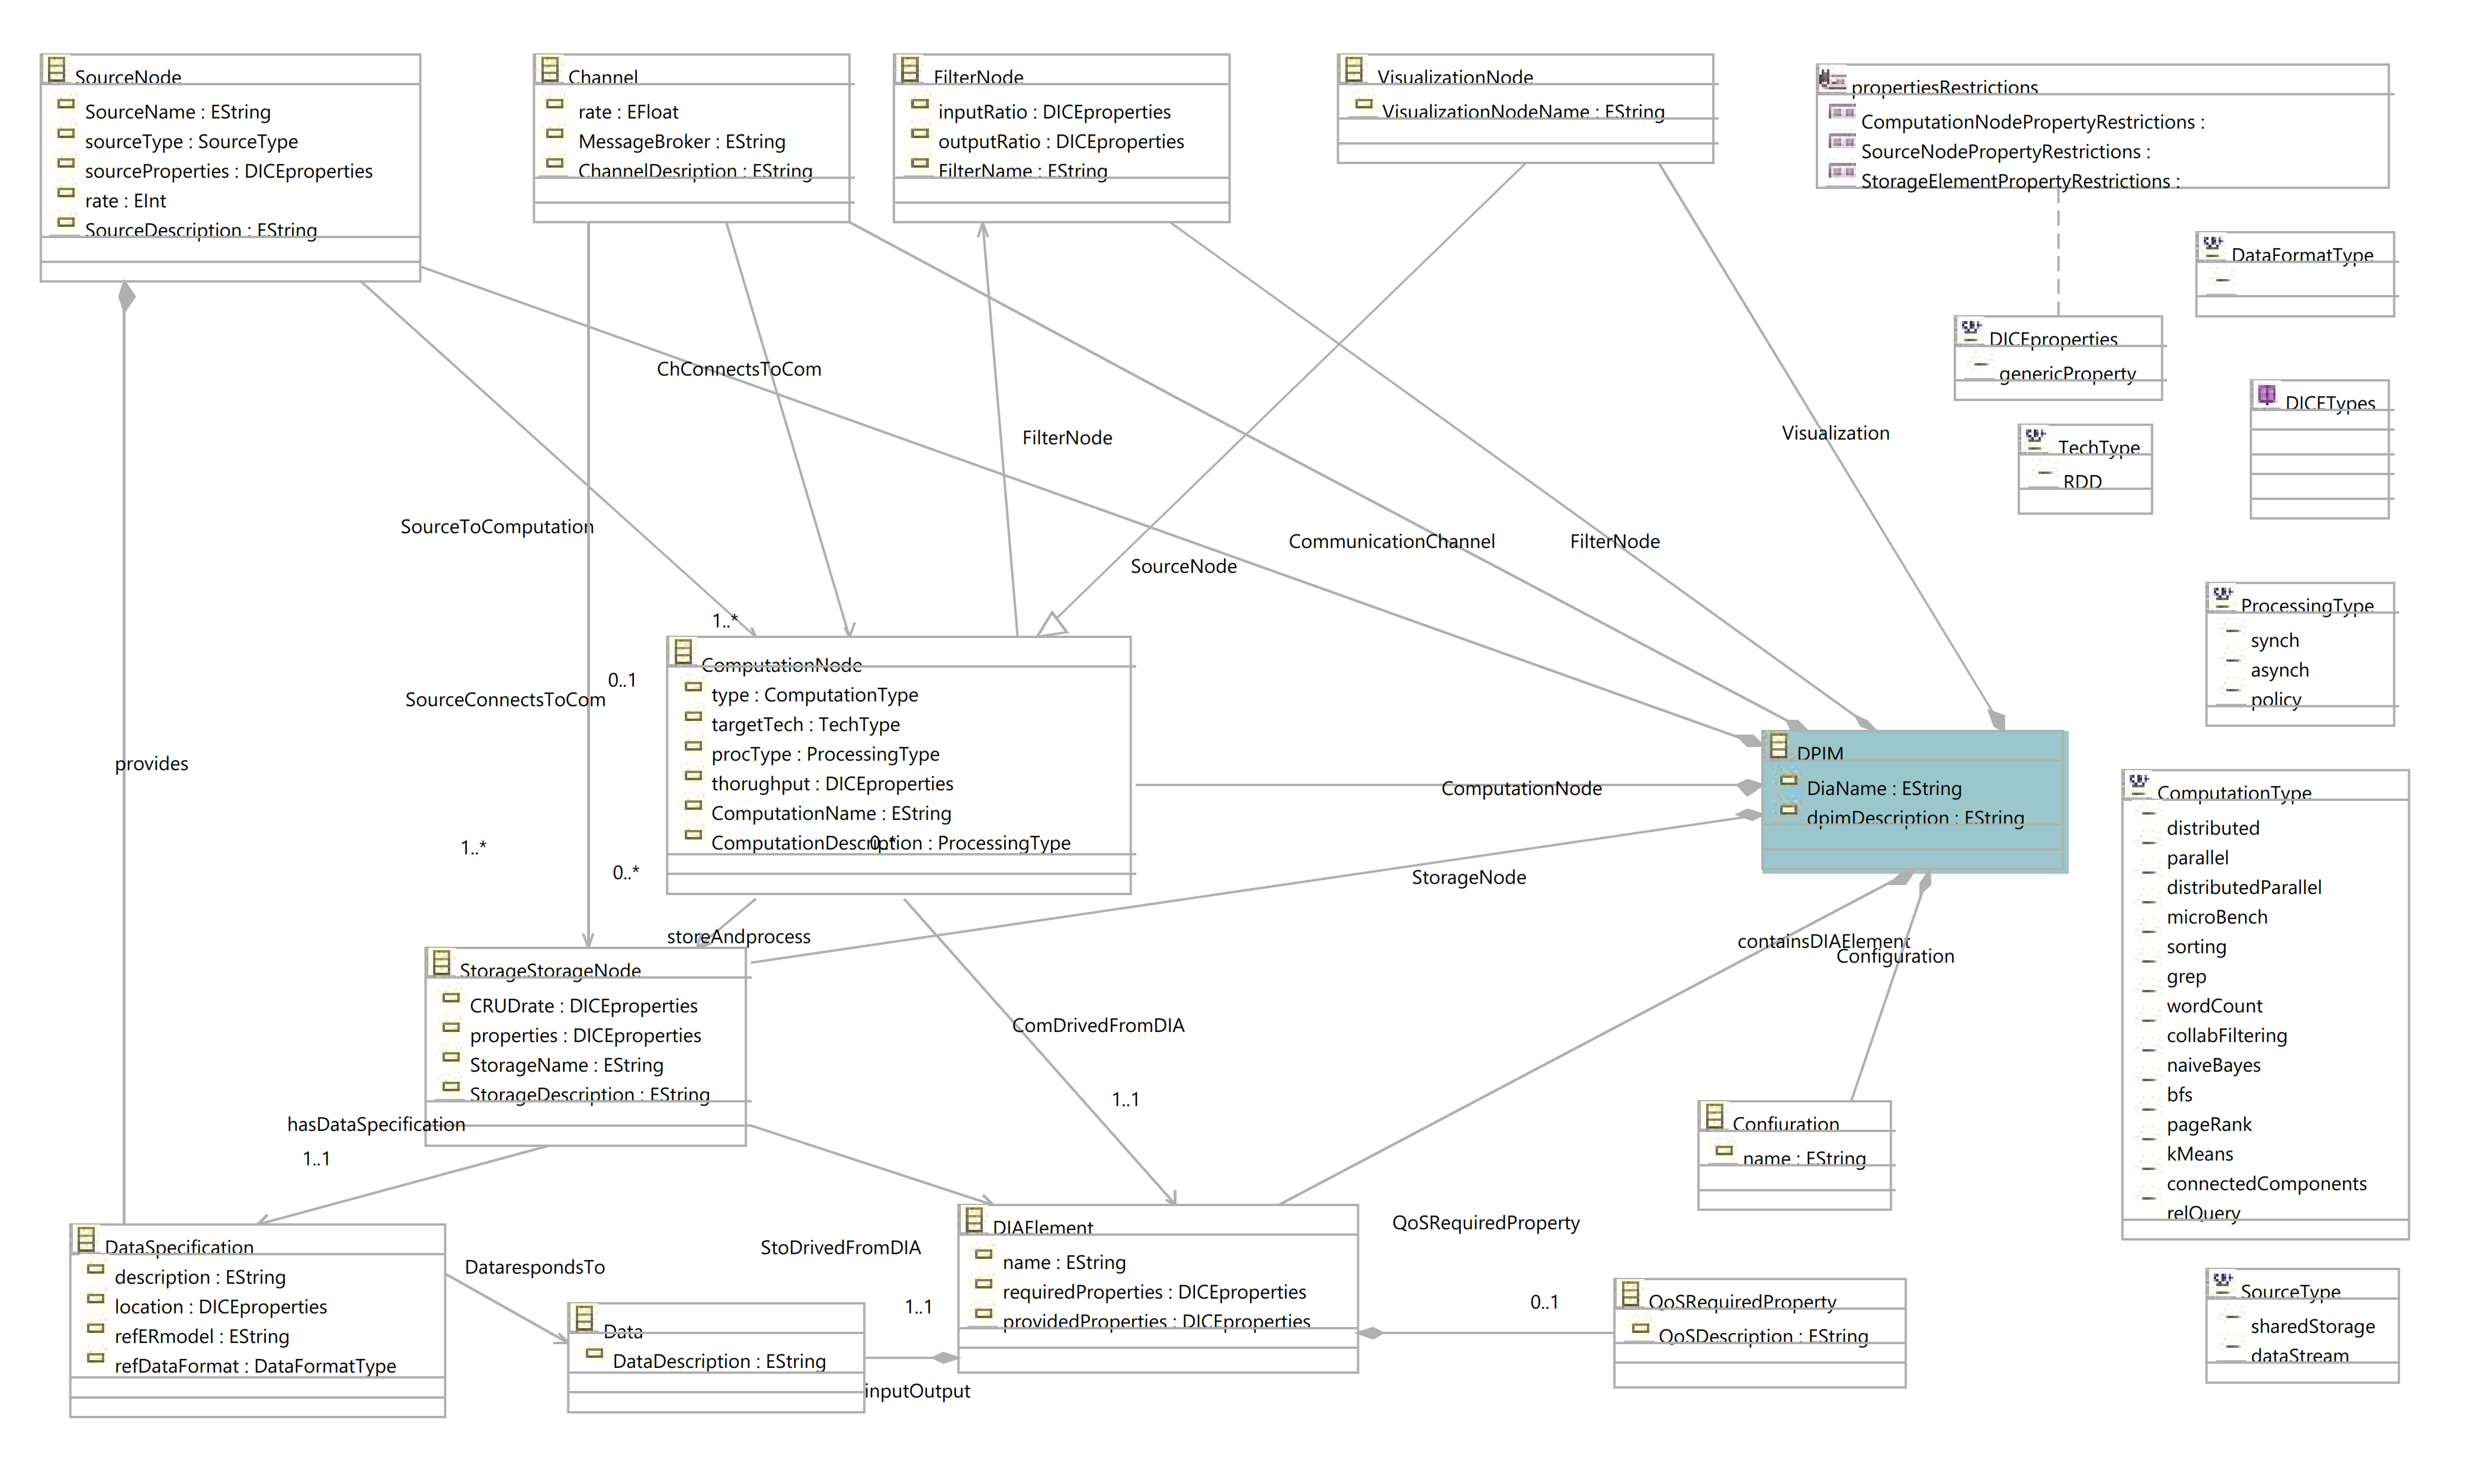
\includegraphics[width=\textwidth]{Images/11.png}
%\caption{\label{fig:metamodel2}DICE DPIM metamodel in portrait form.}
%\end{figure}

%Here is the command to refer to another element (section, figure, table, ...) in the document: \emph{As %discussed in Section~\ref{sect:overview} and as shown in Figure~\ref{fig:metamodel}, ...}. Here is how to %introduce a bibliographic citation~\cite{DAM}. Bibliographic references should be included in a \texttt{.bib} file. 

%Table generation is a bit complicated in Latex. You will soon become proficient, but to start you can %rely on tools or external services. See for instance this \href{https://www.tablesgenerator.com}{https://%www.tablesgenerator.com}. 

% -----------------------------------------------------
\subsection{Product perspective}

    \subsubsection{Scenarios} 
    
        \begin{enumerate}
            
            % - 1 -
            \item \textbf{A student wants to start using the Students\&Companies website}:
            \\Bob is a university student that is looking for an internship to enhance his CV and he decides to exploit a website to facilitate the research, so he connects to S\&C. After entering to the platform for the first time he must register himself on the web application; therefore, he selects the option \textit{"Register as student"} and he fills out sign-up form beginning the registration process providing his email, his full name and creating a password. Bob is then asked to confirm the registration using a link sent on his mailbox and, following the URL, the confirmation is done. At this point Bob will be able to fill out all the information required to complete the account such as \textit{Basic Information}, \textit{Academic Information}, and \textit{Skills and Expertise} (like technical skills, soft skills, and certifications). Bob can also include \textit{Experience and Achievements}, \textit{Internship Preferences}, \textit{CV}, \textit{Portfolio/Projects}, and \textit{Languages Spoken}. Until Bob fills out all the required information he will not be able to use the platform.
            
            % - 2 -
            \item \textbf{A student changes his personal information}:
            \\ Jack has finished some new projects, updated his CV and took a new certification. He logs into S\&C to update his personal information. There he can modify many fields and save the changes. 
            
            % - 3 -
            \item \textbf{A company changes his personal information}:
            \\ The company WeInnovate decides to update his profile on S\&C. On the profile page, it can make changes on the company information.  
            
            % - 4 -
            \item \textbf{A company wants to start using the Students\&Companies website}:
            \\Bridgenix is a company that is looking for interns for an internship that want to offer and it decides to exploit a website to facilitate the research, so it connects to S\&C. After entering to the platform for the first time it must register itself on the web application; therefore, it selects the option \textit{"Register as company"} and it fills out sign-up form beginning the registration process providing its company email, its name and creating a password. The enterprise is then asked to confirm the registration using a link sent on its mailbox and, following the URL, the confirmation is done. At this point Bridgenix will be able to navigate on the homepage and to access to its personal profile in which it can fill out all the information required to complete the account such as \textit{Basic Information} and \textit{Internship Program Details}. The company can also include \textit{Testimonials} from former interns or current employees, enhancing its profile by showcasing the company culture and employee experiences.
            
            % - 5 -
            \item \textbf{A company wants to post a new internship and review student applications}:
            \\After setting up its profile, Bridgenix can post available internships by navigating to the internship creation section. Here, the company can specify details in the \textit{Internship Role Description}, including the title, responsibilities, required skills, qualifications, and the application process.
            It can also provide \textit{Application Details}, to guide students on how to apply for the internship, specifying any required documents. Additionally, Bridgenix may list \textit{Perks and Benefits} associated with the position, such as compensation, additional benefits, and other perks to make the role more attractive to prospective interns. Once the company has fully set up the internship details, it can publish the opportunity on the platform. 
            Every time a student applies for the position, Bridgenix will receive a notification, allowing the company to review the application submitted. For each candidate, the enterprise can access complete details, and if is interested, initiate the selection process to begin evaluating the applicant.
            
            % - 6 -
            \item \textbf{A student proactively searches for an internship}:  
            \\Anita is a student registered to S\&C. Once she is logged into the platform, she can easily find the \textit{Available job search} button. By clicking it, the student will be redirected to another page of the website where she can type into the search bar specific keywords or she can apply specific filters on the search. After issuing the search, Anita will see a list of all the suitable internship positions with synthetic details about the company which is offering it. If she clicks one of them, she will be able to see more details on it.
            
            % - 7 -
            \item \textbf{A company looks for a match}   
            \\The company WorkInc is registered to the platform and has some open positions for internships. The person who is logged in for the company can click the button \textit{"Match Internship"} on the page of a specific internship, then the platform runs analytics to match it with as many students as possible. Internship pages feature a section \textit{"Matching Candidates"} where there is a list of all the suitable candidates for the positions. 
            
            % - 8 -
            \item \textbf{Users interact in the application process}
            \\ The company JobCo has to evaluate some selected students who applied to one of his internships. JobCo will create and upload on the platform timed or not quizzes or questions for the students. The students will submit their answer on the platform. Based on the answers JobCo will extend an offer to the best students, wait-list some others and reject all the other. The students can accept or refuse the final offer made by the company or acknowledge the fact that they were wait-listed or rejected.
            
            % - 9 -
            \item \textbf{Users keep track of the internship }
            \\ The company JobCo can leave private notes to the student, including suggestions, criticisms but also news about the internship. On the other hand, Tony, the student who is carrying out the internship, can communicate problems. Both JobCo and Tony can see the status of the internship and read information regarding the internship, that either one of the two has written on the platform.
            \item \textbf{A university wants to start using the Students\&Companies website}:
            Mordor Institute of Technology is a university that would like to monitor the internships of its students, connects to S\&C. After entering to the platform for the first time it must register itself on the web application; therefore, it selects the option \textit{"Register as university"} and it fills out sign-up form beginning the registration process providing its university email, its name and creating a password. The university is then asked to confirm the registration using a link sent on its mailbox and, following the URL, the confirmation is done
            
            \item \textbf{Universities monitor the internships of their students }
            \\ The university of Erewhon has a list of all the students enrolled to it that are doing an internship. The university can further look into the internship and getting to know the details of it (the company, the duration, location, role title, etc.). However, the university can look the status of an internship only once it is started, not before.
        \end{enumerate}
        
        \newcommand{\mycomment}[1]{}
        \mycomment{
            \begin{enumerate}[label=\textbf{[\arabic*]}, left = 0 pt, align = left]
            % ----
            \item \textbf{A Student Registers on the Platform}:             % DONE
            \\A student that is looking for an internship visits the S\&C platform for the first time. He or she decides to register to access potential internship opportunities.
            They enter the Homepage and clicks on \textit{"Sign Up"}. At this point, a form appears where the student must insert his email, creates a password, and fills in their personal and academic details. After submitting the form, they quickly receive an email confirmation and follow the link to activate their account. 
            Excited to start his search, the user logs in and begins creating his profile to make himself more visible to companies.
            
            % ----
            \item \textbf{Company Registration}:                            % DONE                     
            \\A company that is looking for interns visits the S\&C platform for the first time. It decides to register so it can access potential internship candidates. 
            It enters the Homepage and clicks on \textit{"Sign In"}. At this point a form appears where the enterprise must insert the company name, the company email and creates a password. After submitting the form, it quickly receives an email confirmation and follows the link to activate its account. 
            Excited to find the right candidates, the company logs in and begins creating its profile to make its internships more visible to prospective interns.
            
            % ----
            \item \textbf{Student Profile Creation}:                        % DONE
            \\Once a student logs into the platform, they can click on the \textit{"Edit profile"} button, which will redirect to a dedicated webpage displaying all the information required for the registration, along with a form that they can fill out. The student can add \textit{Basic Information}, \textit{Academic Information}, and \textit{Skills and Expertise} (like technical skills, soft skills, and certifications).
            They can also include \textit{Experience and Achievements}, \textit{Internship Preferences}, \textit{CV}, \textit{Portfolio/Projects}, and \textit{Languages Spoken}
            
            % ----
            \item \textbf{Company Profile Creation}:                        % DONE
            \\Once a company logs into the platform, it can access to its profile by clicking on the icon in the
            top-right corner of the screen. This directs the company to its profile page, where it can select the \textit{"Edit Profile"} button to add or modify information. Here, the company can fill details to personalize its profile, such as \textit{Basic Information} and \textit{Internship Program Details}.
            The company can also include \textit{Testimonials} from former interns or current employees, enhancing its profile by showcasing the company culture and employee experiences.
            
            % ----
            \item \textbf{Internship Posting by Company}:                   % DONE       
            \\After setting up its profile, the company can post available internships by navigating to the internship creation section. Here, it can specify \textit{Internship Role Description} details, including the role title, responsibilities, required skills and qualifications, and the application process.
            The company can also provide \textit{Application Details}, which feature an \textit{"Apply Now"} button for candidates and any required documents. It may also list \textit{Perks and Benefits} associated with the internship, such as compensation, additional benefits, and other perks to make the position more attractive to prospective interns.
            
            % ----
            \item \textbf{A Student Proactively Searches for an Internship}:  % DONE                 
            \\Anita is a student registered to S\&C. Once she is logged into the platform, he or she can easily find the \textit{"Available job search"} button. By clicking it the student will be redirected to another page of the website where they can type into the search bar specific keywords or they can apply specific filters on the search. After issuing the search, she will see a list of all the suitable internship positions with synthetic details about the company which is offering it. If she clicks it, she will be able to see more details on it.
            
            % ----
            \item \textbf{A Student Actively Searches for a Match}:     % TO SEE              
            \\Tom, a student registered to the platform, fills or updates his/her profile with his information, he or she can click the button \textit{"Match me"} on his profile. Then, the platform runs analytics to match it with as many companies as possible. Profiles of students feature a section with \textit{"Matching Internships"} where there is a list of all the suitable internships for him/her.
            
            % ----
            \item \textbf{A Company Looks for a Match}                  % DONE
            \\The company WorkInc is registered to the platform and has some open positions for internships. The person who is logged in for the company can click the button \textit{"Match Internship"} on the page of a specific internship, then the platform runs analytics to match it with as many students as possible. Internship pages feature a section \textit{"Matching Candidates"} where there is a list of all the suitable candidates for the positions.
            
            % ----
            \item \textbf{Student Application to Internship}                      
            \\Once a student finds an internship that might interest them, they can click on the preview of the placement, which will redirect to the company's private webpage. By pressing the \textit{"Apply Now"} button, a form will appear where the student must enter all the required information specified by the company. Once all the fields are completed, they can submit their application by clicking the \textit{"Submit"} button.
            
            % ----
            \item \textbf{Company Review of Student Applications}           % DONE 
            \\Once a company has posted one or more internship proposals, it will be able to see the applications submitted for each proposal by clicking on \textit{"Sent applications"}, which will redirect to a dedicated webpage displaying all the applications for a particular internship. For each application, brief information is shown on the screen, and the company can access the complete details by clicking the \textit{"More details"} button. If the company is interested to the student, it can click on \textit{"Start Selection Process"} to begin evaluating the candidate and will be prompted a calendar to indicate the available days and time slots.
            
            % ----
            \item \textbf{Student Interview Scheduling}  
            \\When a contact between a company and a student is established, the student will be able to choose one day from a list of available dates to conduct the interview.
            \item \textbf{Interview Conducted by Company}                        
            \\ Sarah, a student who was able to schedule an interview, will be asked a set of questions in a certain amount of time. The time and questions are decided by the company.
            \item \textbf{Company Selection of Candidate}                        
            \\
            \item \textbf{Internship Offer Extended to Student}                  
            \\
            \item \textbf{Internship Offer Acceptance by Student}                
            \\
            \item \textbf{Feedback Submission by Student Post-Internship}        
            \\
            \item \textbf{Feedback Submission by Company Post-Internship}        
            \\
            \item \textbf{Statistical Analysis of Internship Matches}            
            \\
            \item \textbf{Internal Status Update by Student}                     
            \\
            \item \textbf{Internship Status Update by Company}                   
            \\
            \item \textbf{Notification of New Internship Opportunities}          
            \\
            
            \end{enumerate}
        }
    
    % -----------------------------------------------------.
    \newpage
    \subsubsection{Domain Class Diagram}
    To capture the different classes, their methods and their interactions we drew the following domain class diagram
        \begin{figure}[h!]
            \centering
            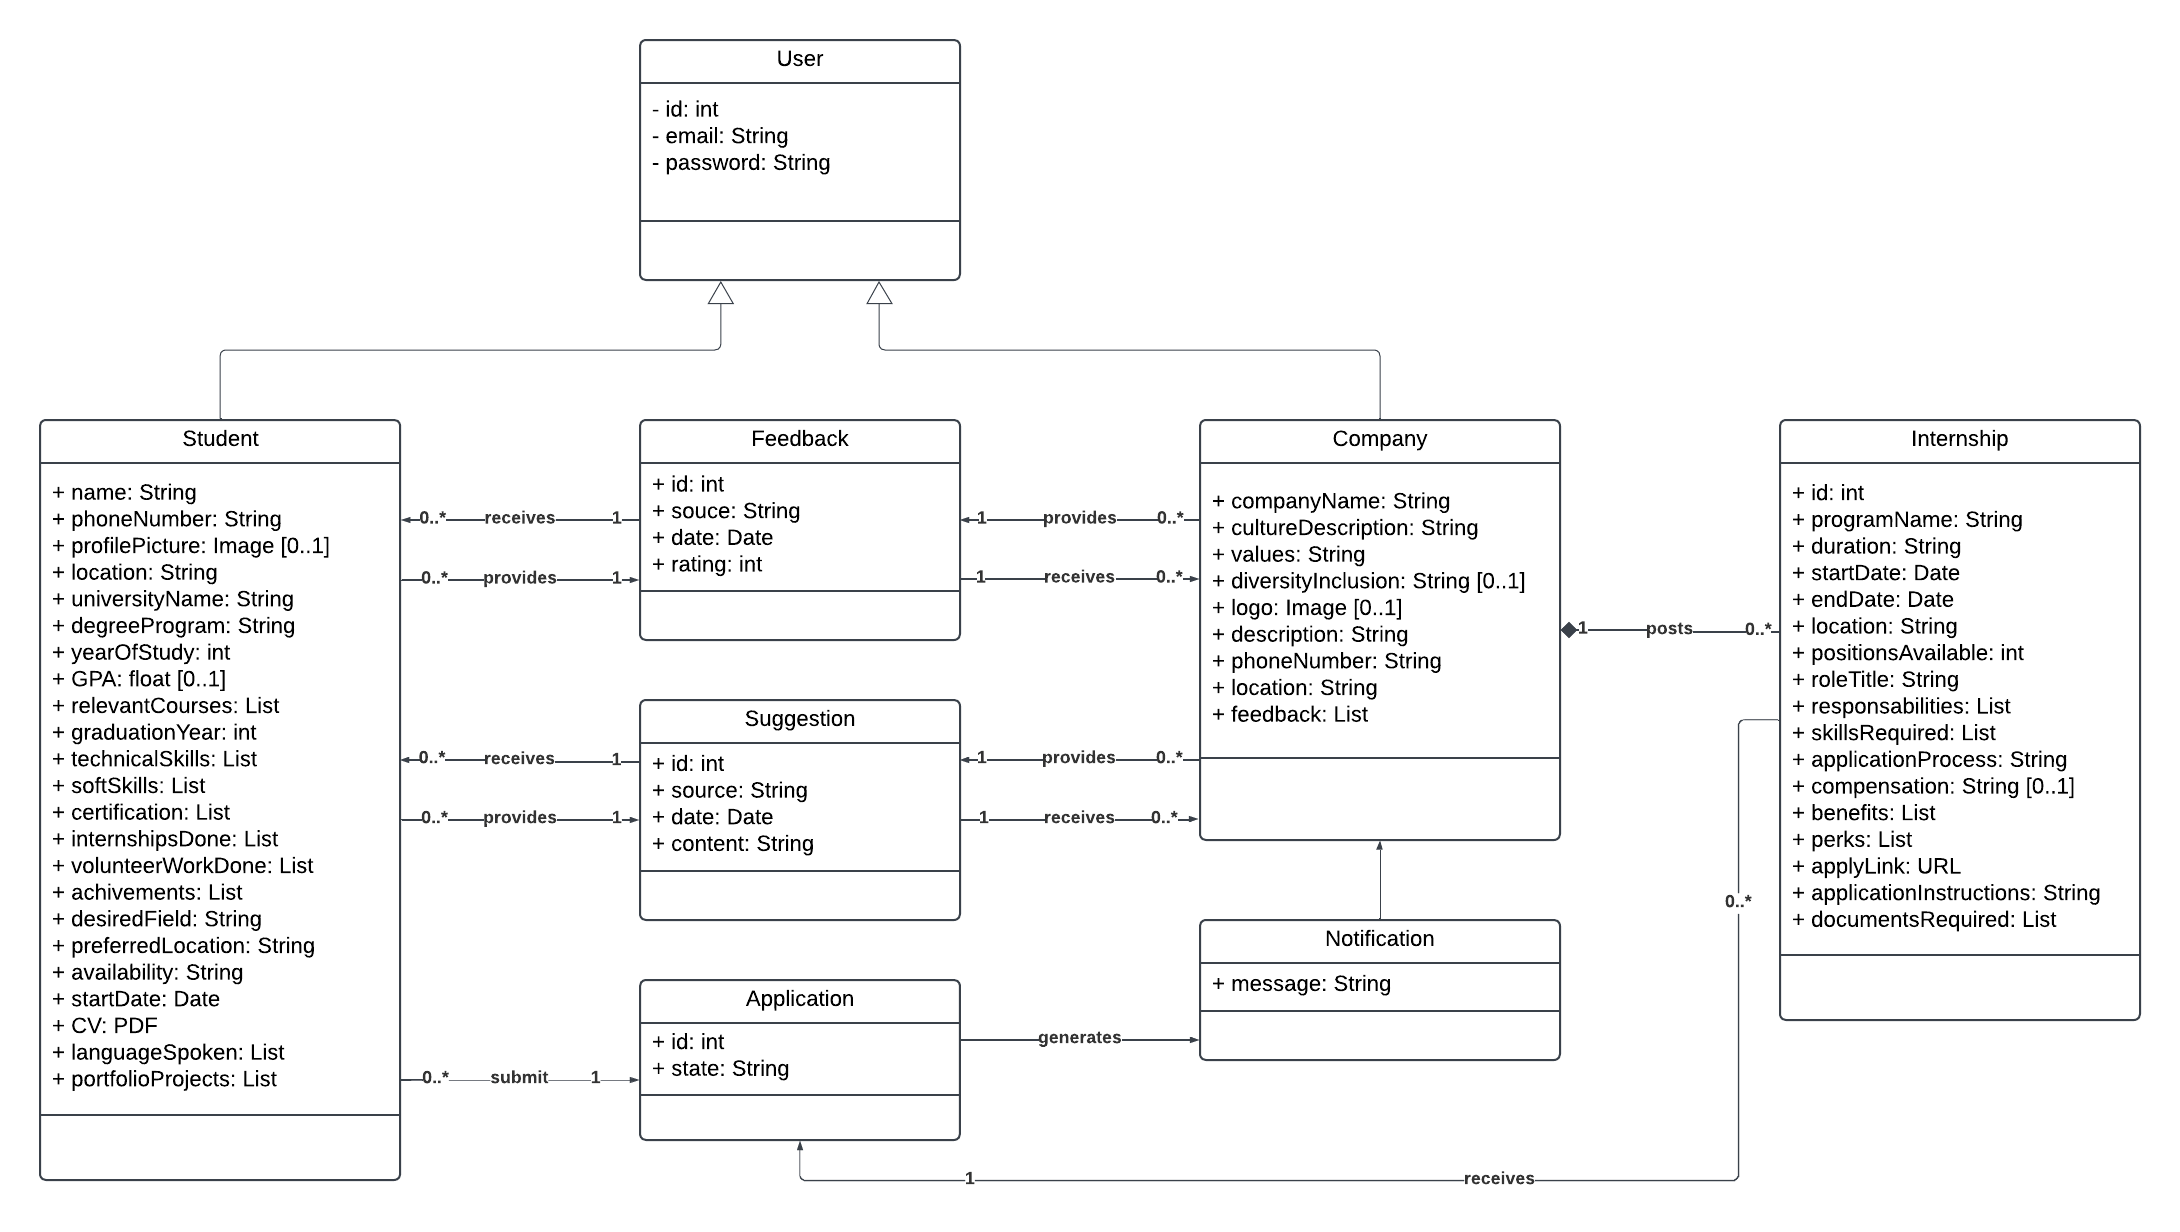
\includegraphics[width=1\textwidth]{RASD/Images/ClassDiagram.png}
            \caption{Class Diagram}
            \label{fig:example}
        \end{figure}
    
    
    % -----------------------------------------------------
    
    \subsubsection{State Diagrams}
        The most crucial aspect of the application is the creation and evolution of the internship positions on the platform. Not to leave any room for doubts, we explain both the point of view of the company and the one of the student.
        \\
        A company can close an internship position whenever it wants to. Once it closes the internship, the applications who were accepted but not confirmed or not refused, the pending applications, and the applications needing an further assessments are automatically rejected. Instead, for those who confirmed, we consider the moment of the closing of the open position by the company as the moment in which they start their internship.
        \\
        The following is the point of view of the company
        \begin{figure}[h!]
            \centering
            
\includegraphics[width=1\textwidth]{RASD/Images/CompanyPOV.png}
            \caption{The evolution of an internship position on the platform from the point of view of a company}
            \label{fig:example}
        \end{figure}
        \\
        The following one, instead, is the point of view of a student:
        \begin{figure}[h!]
            \centering
            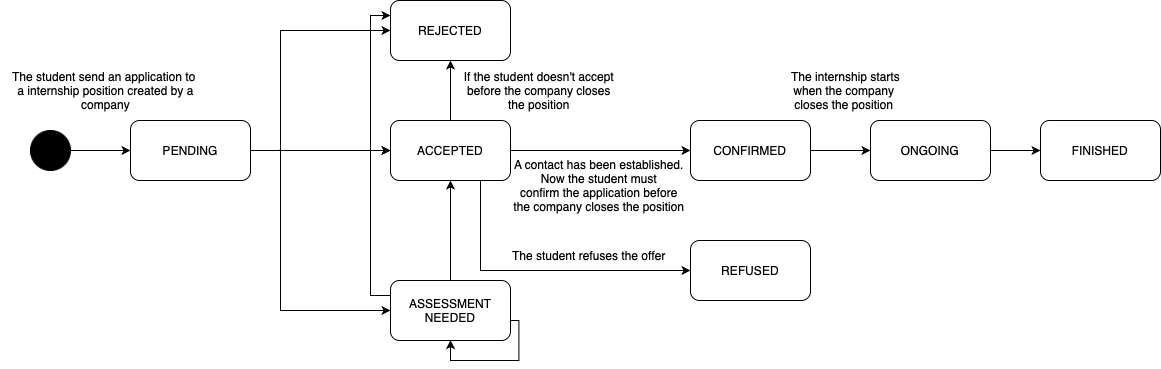
\includegraphics[width=1\textwidth]{RASD/Images/StudentPOV.png}
            \caption{The evolution of an internship position on the platform from the point of view of a student}
            \label{fig:example}
        \end{figure}
        

% -----------------------------------------------------


\subsection{Product Functions}
    \begin{enumerate}
        \item \textbf {Sign Up and Log In}
        \\ The users sign up to the platform by providing an email and a password. A registered user logs in to the platform by providing the same information. At the moment of sign up it is necessary to indicate whether the account is related to a company or to a student, since the two types of account are treated differently inside the platform.
        \item \textbf {Profile Information Filling}
        \\ The users fill his profile information. Companies will be asked for its name, the headquarters location, approximated number of employees, CEO, sector in which it operates and it can also include testimonials from former interns or current employees, showcasing the company culture and employee experiences. Students will be asked for name, surname, education, work experience, skills and CV. A part of the information is published on the platform, another part of the information is used by the recommendation system.
        \item \textbf {Internship Position Creation}
        \\ Companies can create new internships positions by establishing the expired deadline to apply, the work place, the role title, the responsibilities, the required experience, the required skills and the salary range.
        \item \textbf {Management of the Selection Process}
        \\ Companies see the profiles of students who applied to an internship. S\&C enable them to configure the selection process based on their needs. They can reject students who applied to an internship position after checking their qualifications on their profiles; they can directly accept one or more of them. Companies can propose dates of tests to assess the preparation of students who applied for an internship position and finalize the decisions after the tests or requesting an online interview.
        \item \textbf {Communication Space}
        \\ After an internship is started, both the students and companies have dedicated sections of the website to exchange information, communicate problems, indicate suggestions, make announcements (all regarding the internship) such that both of the interested parties can benefit from the sharing of information. 
        \item \textbf {Feedback Management}
        \\ After the internship is finished the platform asks both the company and the student to rate and review each other. Moreover it asks both parties for suggestions. Collecting this kind of information is particularly important to feed and improve the recommendation system.
    \end{enumerate}


% -----------------------------------------------------

\subsection{User Characteristics}
    Users of S\&C are divided into two distinct categories:


% -----------------------------------------------------

% one subsubsection for each type of user
\subsubsection{Students}
    They can search for an internship, get suggested internships, apply to open positions, participate in the selection process and give feedback about an internship for which they were selected.


% -----------------------------------------------------

\subsubsection{Companies}
    They can create internship openings, advertise them, set up the selection process, track the ongoing status of the internships and give feedback about students who undertook one of their internships.


% ------------------------------------------------------
\subsubsection{Universities}
    They can monitor the internships of their students and get details on them.
% ------------------------------------------------------
\subsection{Assumptions, Dependencies and Constraints}


% ------------------------------------------------------

\subsubsection{Regulatory Policies}
    Personal information will be processed in compliance with GDPR rules.


% ------------------------------------------------------

\subsubsection{Domain Assumptions}
    \begin{enumerate}[label={[D\arabic*]}]
        \item {Students insert correct information about their skills and experience}
        \item {Students do not cheat when taking skill assessment tests}
        \item {Students apply to jobs in countries where they have a work permit}
        \item {Students provide valuable feedback when asked for it}
        \item {Companies offer existing and legal contracts for the internships}
        \item {Companies insert correct information about the internships}
        \item {Companies periodically review information about the internship candidates}
        \item {Companies prepare proper skill assessment test to evaluate candidates}
        \item {Companies provide valuable feedback when asked for it}
        \item {Most of universities are contacted before the website is online so that most of them are already present on the platform, when the website is deployed}
    \end{enumerate}